%\documentclass[11pt]{article}
\documentclass[11pt,usenames,dvipsnames]{article} %added color definition
\usepackage{cite}

%%% PAGE DIMENSIONS
\usepackage{geometry} % to change the page dimensions
\geometry{a4paper, margin=3cm} % or letterpaper (US) or a5paper or....
% \geometry{margin=2in} % for example, change the margins to 2 inches all round
% \geometry{landscape} % set up the page for landscape
%   read geometry.pdf for detailed page layout information

\usepackage{graphicx} % support the \includegraphics command and options

\usepackage[parfill]{parskip} % Activate to begin paragraphs with an empty line rather than an indent

%%% PACKAGES
\usepackage{booktabs} % for much better looking tables
\usepackage{array} % for better arrays (eg matrices) in maths
\usepackage{paralist} % very flexible & customisable lists (eg. enumerate/itemize, etc.)
\usepackage{verbatim} % adds environment for commenting out blocks of text & for better verbatim
%\usepackage{subfig} % make it possible to include more than one captioned figure/table in a single float. CGW: incompatible with subcaption
% These packages are all incorporated in the memoir class to one degree or another...
\usepackage{cite} %CGW use bibtex to cite sources
\usepackage{xcolor} %CGW change text color
%\usepackage{subfigure} %CGW creates subfigures.  incompatible with subcaption
\usepackage{caption} %CGW
\usepackage{subcaption} %CGW include subfigures
\usepackage{amsmath} %CGW: equations
\usepackage[utf8]{inputenc} %CGW: list of tables
\usepackage{appendix} %CGW: appendices formatting
\usepackage{tabularx} %CGW: automatic line break
\usepackage{float} %CGW force placement of figure
\usepackage{colortbl} %CGW cell colors in excel2latex conversion
\usepackage{rotating} %CGW text rotation in excel2latex conversion
\usepackage{longtable} %CGW multipage table
\usepackage{multirow} %CGW multirow for excel2latex
\usepackage{rotating} %CGW rotated text for excel2latex

%%% HEADERS & FOOTERS
\usepackage{fancyhdr} % This should be set AFTER setting up the page geometry
\pagestyle{fancy} % options: empty , plain , fancy
\renewcommand{\headrulewidth}{0pt} % customise the layout...
\lhead{}\chead{}\rhead{}
\lfoot{}\cfoot{}\rfoot{\thepage}

%%% SECTION TITLE APPEARANCE
\usepackage{sectsty}
\allsectionsfont{\sffamily\mdseries\upshape} % (See the fntguide.pdf for font help)
% (This matches ConTeXt defaults)

%%% ToC (table of contents) APPEARANCE
\usepackage[nottoc,notlof,notlot]{tocbibind} % Put the bibliography in the ToC
\usepackage[titles,subfigure]{tocloft} % Alter the style of the Table of Contents
\renewcommand{\cftsecfont}{\rmfamily\mdseries\upshape}
\renewcommand{\cftsecpagefont}{\rmfamily\mdseries\upshape} % No bold

%%% List of Figures setup 
%%% https://tex.stackexchange.com/questions/475767/list-of-tables-and-list-of-figures-error-when-using-caption
\captionsetup[subfigure]{list=true}
\usepackage[subfigure]{tocloft} %http://mirrors.ibiblio.org/CTAN/macros/latex/contrib/tocloft/tocloft.pdf
\newcounter{lofdepth}
\setcounter{lofdepth}{3}
%\cftpagenumbersoff{subfigure}

%List of Tables setup
\newcounter{lotdepth}
\setcounter{lotdepth}{2}

%%% Hyperlinks
\usepackage{hyperref}
\hypersetup{
	colorlinks=true,
	linkcolor=blue,
	filecolor=magenta,
	urlcolor=ForestGreen,
}

%%% Variables
\title{%
	An open source spatial news web app development project \\
	\large Masters in GIS\&S Thesis Proposal\\
}

\author{Callie Wentling\\
	\small Advisor: Professor Marco Painho, Ph.D}
\date{} % Activate to display a given date or no date (if empty), otherwise the current date is printed 

\begin{document}
%\pagenumbering{roman} %Use for longer front matter (title page, abstract, longer table of contents, thanks, etc.)

\maketitle
\thispagestyle{empty} %Removes page number from this page
%{\color{red}
%	To do:
%	\begin{itemize}
%%		\item Remove bullet points from relevant terms
%%		\item Hyperlink
%%		\item Add remaining appendices
%%		\item Create reference document for figures, tables, etc.
%%		\item Rewrite Grant sessions that don't apply to the NOVA proposal
%%		\item Check the proposal format for NOVA
%%		\item Check the goals for the HOW TO WRITE A THESIS proposal (google drive)
%%		\item Create reference section on Mendeley and import into doc
%%		\item Visualize mendeley references in doc
%%		\item recover literature review structure in to document and cite relevent references
%%		\item Write
%		\item Specifications
%	\end{itemize}
%}

\vspace*{\fill}
\section*{Project summary}
This project seeks to develop a proof-of-concept (POC) open source (OS) and free software (FS) web application (Web App) that supports the visualization of the spatial distribution of news story contents (“incidents”), as well as filtering mechanisms for improved temporal, spatial, and thematic investigation of news articles. This geospatial element is expected to provide an additional dimension of understanding that allows users to better contextualize news stories, search repositories, or monitor spatial/temporal trends at a community level (within a city). In addition to the aforementioned improvements of user experience for the public (readers, researchers, and monitors), it is also expected to support publishers via the inference of new insights from their existing internal data, such as the illumination of under- or over-reporting of areas by theme for better investigative coverage. Ideally, this functionality could be expanded to integrate multiple sources, as well as the incorporation of planned events and/or resources to provide a more comprehensive understanding of one's surroundings in both the planned future and transpired past.

\newpage
\thispagestyle{empty} %Removes page number from this page
{\small
\tableofcontents
}

%\newpage
{\small
\listoffigures
}

%\newpage
{\small
\listoftables
}

\newpage
\pagenumbering{arabic}
\section{Framework}  \label{sec:framework}
%{\color{red} Enquadramento: 2 páginas}
The ongoing COVID pandemic has highlighted the value of the visualization of information on a map, not only for specialists to monitor and predict viral outbreaks, but to arm the public with empowering information as well. Of course, the value of geographic information systems (GIS) goes beyond public health services and is already nestled into our everyday activities in the form of daily tasks such as navigation and service selection. Applications like Google Maps, AirBnB, and UberEats allow non-technical users to visualize and filter the distribution of various services through spatial (SA), temporal (TA), and thematic attributes (ThA). For example, a user on AirBnB may filter all apartments with high speed wifi (ThAs) available in the Estrela neighborhood and within walking distance to a market (SAs) from Aug 1 to Aug 7, 2020 (TA).

Yet, though this type of manipulation is commonplace in the products of many industries, it is glaringly absent from that of news media.  When reading about an incident occurring in an unfamiliar place, readers will often need to look up the location. They may have trouble relating the spatial significance of an incident to neighboring occurrences or historical events in the same spot. Many articles define place via textual descriptions, but these can be easily overlooked if searched by keyword, especially if different names or alternate designations are employed by the searcher.  This is a problem for researchers who may want to define a study area that does not conform to traditional administrative boundaries or existing points of interest, but also for the casual user or city official.  The former might, while perusing headlines, miss an article of interest relating to a place along their commute home from work. The latter could be an elected official who seeks to monitor an issue (such as gentrification or homelessness) but is unable to visualize the subtle distribution of such events throughout his or her district. In these cases, as well as a host of others, there is obvious disconnect between the existence of data and its usability.  As such, there is operational as well as academic value in better understanding the spatial distribution of events within a community, such that additional informative insights can be drawn.  

This project seeks to develop a set of functional tools that supports the creation and management of a spatial database of news stories, a publishing interface (associating place and adding records to the database), a user interface (list and map format search, filter, and visualization of results from the database), as well as a story visualization plugin (a map displaying the distribution of a story in a contextual map per story page).  See Section \ref{sec:objectives} for more details. This proof of concept (POC) functionality should demonstrate the value of new spatial products in news media, and provide a basis from which meaningful projects may be developed for mass media applications in the future.

\textit{Note: The project proposed here is not one of automatic place extraction from existing news stories. See Appendix \ref{appendix:existing_projects} for more details.}


\subsection{Study area}

The project will use a  study area (news story data from at least one section of a publication for a defined time interval) of Lisbon, Portugal (such as “Local” in Público for Q3 of 2020) %and one in the USA (such as “Colorado News” from The Denver Post for the same time period). 
 In the case that opportunities to include additional study areas such as other cities, sections of publications, or additional sources of incident data (such as information from other newspapers or municipalities) arise, these may be accommodated as well, time allowing. By building a tool specific to Lisbon, the project seeks to accommodate the culture and business processes of the local community, providing a platform that is useful and valuable to users (whether citizens, local officials, researchers, or publishers). 

\subsection{Languages}

The Web App should support the definition of use in English and Portuguese (leveraging a platform for expansion to other languages) for all elements of the user interface (such as project description, instructions, filters, units, etc.). All data incorporated from external sources (such as news article contents, publisher tags, gazetteer names, etc.) may remain in their original forms/languages (though alternate forms will be supported if provisioned by the original source). The language options of English and Portuguese should support the international use and cross-investigation of a wider user base.

\subsection{Access to results}

The project results will be licensed as free and open source such that these can be accessible and leveraged by other individuals or organizations for further development or related projects. Wherever possible, the project will leverage existing open source tools, platforms, and data. However, agreements with data providers may require restriction from public access of their proprietary data. 

\subsection{Sustainability}
The project is a foundation for future development in the geospatial and temporal distribution of news story contents.  The proof of concept should demonstrate the value of such filtering and may be built upon in one or more of the following ways: 
\begin{enumerate}
	\item as a free tool; 
	\item as the base of a new online news journal product;
	\item incorporated into existing online databases to incorporate the temporal spatial dimension into and enhance their own thematic tools; or 
	\item to be incorporated into municipalities as a public participation platform / community empowerment tool to better understand incidents that are spatially relevant. 
\end{enumerate}

This last option is especially interesting if future planned events and city data are layered in. It is also the direction of most interest to me and future efforts may involve collaboration with one or more cities to design a public participation tool. Additional functionality may include additional languages, additional study areas, development of a smart phone application, an option for automatic localization (such as for geo-tagging news stories or proximal searching), incorporation of historical datasets, incorporation of future events, additional data visualization options, APIs for integration with other applications, white-labeling options for commercial applications, etc.

At minimum, its documentation and codebase will be available under an open license from which anyone may develop in the future.

\subsection{Impact}
\begin{enumerate}
%	\item 1+ news publication organizations
	\item 1 webapp, freely and openly accessible, available in English and Portuguese languages
	\item 1 webapp development code, open licensed for further or related future development by any individual or organization.
\end{enumerate}


\section{Hypothesis} \label{sec:hypothesis}
%{\color{red} Hipóteses de trabalho: 1 páginas}
The goal of this project is to explore if there is a value to plotting the spatial distribution of news story contents, as well as provide users a portal through which to interact with the data to extract the desired information.  

It is expected that the association of specific place (potentially non-conforming to existing administrative boundaries or defined points of interest) to traditional news articles will provide an added dimension of understanding to communities at a local level. Users will find additional insights from the ability to view or filter spatial attributes, especially in conjunction with thematic and temporal attributes. This type of data preparation, though it is initially cumbersome to establish and requires adjustment of publishers' processes to maintain, will provide a powerful foundation from which future economic (improved publisher products elevating their offering and attracting/maintaining a customer base), societal (illumination of local trends requiring intervention, improved community engagement of readers with their surroundings, or improved city resources), and academic (improved research functionality) benefits may stem.  If this type of functionality and improved user experience are well-implemented by a handful of productive news services, it will force a shift of the industry standard towards integration of spatial attributes and spatially related products.

Though testing of these hypotheses through rigerous comparison to the status quo (traditional online news sources without a spatial element) and emerging product performing automatic extraction of place (such those of the GDELT project, Section \ref{appendix:existing_projects}) are not included in this endeavor, the resulting tools should provide a basis from which future projects may develop and evaluate.

\section{Objectives} \label{sec:objectives}
%{\color{red} Objetivos: 1 página}
The proposed tangible results are a web application (Web App) that allows non-technical users to explore spatial and temporal incident distributions within the chosen study areas.  Its functionality includes:
\begin{enumerate}
	\item A spatial database of incidents that supports the association of spatial, temporal, and thematic attributes. See Appendix \ref{appendix:organization}/Figure \ref{fig:data_model} for preliminary data model.
	\item A POC Input tool for publishers that allows users to define the place(s) (via search for existing administrative boundaries and points of interest [POIs] through existing gazetteers or definition of new polygons or points via drawing) as well as time of occurrence of incidents. It shall also, of course, preserve or potentially improve upon the association of traditional thematic attributes and keyword search. See Appendix \ref{appendix:organization}/Figure \ref{fig:input_ui} for preliminary \textit{Input} layout.
	\item A POC Context map (visualization of an incident on a local map) for integration into each article page. See Appendix \ref{appendix:organization}/Figure \ref{fig:context_ui} for preliminarsy \textit{Context} layout.
	\item A POC Search tool for researchers that allows users to filter by spatial (one or multiple defined places or via drawn definition of the study area), temporal, and or thematic attributes. The results should be displayable via both map and list views, as well as support CSV export functionality. See Appendix \ref{appendix:organization}/Figure \ref{fig:search_ui} for preliminary \textit{Search} layout.
	\item A POC Dashboard tool for monitors (publisher, city officials, etc.) to monitor the spatial/temporal development of incidents according to their settings. 
\end{enumerate}

Beyond the implementation of a POC toolset and demonstration of value, this project also seeks to enhance my skillset and experience in the following ways:
\begin{enumerate}
	\item Planning and execution of a GIS "product"
	\item Creation and maintenance of a geospatial database
	\item Programming of user interfaces
	\item Leveraging of open source programs and tools
	\item Incorporation of multi-lingual functionality
	\item Collaboration with news industry users
	\item Collaboration with city official users
	\item Collaboration with readers users
	\item Leveraging the knowledge and experience on smart cities, public participation, and geospatial services at NOVA
	\item Development of a "smart city" product
	\item Development of open source tools
	\item Provisioning of the base product for future expansion into desired directions (integration of future language options, accommodation of multiple news sources, integration of planned events, integration of city resources, integration of automatically extracted place from historic sources, etc.)
\end{enumerate}

\section{Methodology} \label{sec:methodology}
%{\color{red} Metodologia: 2 páginas}
To support the identified objectives, the following must occur:
 %(see section X for major timeline definitions, some elements are already ongoing or complete):
\begin{itemize}
	\item Perform literature review of prior art and study of existing relevant platforms and tools.
	\item Conduct interviews with stakeholders (publishers, journalists, readers, researchers, and city officials) to establish and prioritize functionality elements.
	\item Finalize specifications, mockups of Web App functionality, data model, and finalization of relevant tools and libraries. 
	\item Initialize the development environment.
	\item Receive data from collaborating journals within the defined study areas.
	\item Establish incident database, accommodating multiple language options. Load gazetteer(s) and relevant administrative boundary data.
	\item Develop and test Input tool.
	\item Develop and test Search tool.
	\item Develop and test Dashboard tool.
	\item Develop and test Context tool.
	\item Translate Web App content to Portuguese and load translations.
	\item Migrate site to the server.
	\item Test among stakeholders.
	\item Compare against mined location results.
	\item Compare against existing media search options.
	\item Document results and plan future development.
\end{itemize}


\section{Preliminary Organization} \label{sec:organization}
%{\color{red} Esboço de organização do TPE (índice)}
{\footnotesize
	\begin{enumerate}
	\item Introduction
	\begin{enumerate}
		\item Context
		\begin{enumerate}
			\item Smart cities \cite{Oliveira2021, Roche2012}
			\item News
		\end{enumerate}
		\item Hypothesis
		\item Objectives
	\end{enumerate}
	\item Literature review
	\begin{enumerate}
		\item Web tools for news
		\begin{enumerate}
			\item News search tools
			\begin{enumerate}
				\item \textit{Portuguese based publication} (ex: Público) \cite{Publico2020}
				\item \textit{US based publication} (ex: The Denver Post) \cite{TDP2020}
				\item \textit{Good example}
				\item \textit{Bad example}
			\end{enumerate}
			\item Automatic extraction of place in news
			\begin{enumerate}
				\item GDELT
			\end{enumerate}
			\item WebGIS as a search tool
			\begin{enumerate}
				\item AirBnB
				\item UberEats
				\item Idealistia
				\item CML
				\item Facebook events
			\end{enumerate}
			\item Open Source
			\begin{enumerate}
				\item Definition of terms
				\item Licensing options
			\end{enumerate}
			\item Open/free formats in WebSIG
		\end{enumerate}
		\item GIS on the Web
		\begin{enumerate}
			\item Open/free code solutions
			\begin{enumerate}
				\item QGIS cloud
				\item ArcGIS Server
				\item Lizmap
				\item Leaflet
				\item MapServer
				\item Geomajas
			\end{enumerate}
			\item Commercial solutions
			\item Design \cite{Parasecoli2019, Fisher2014, Shneiderman2020, Meeks2019, Shneiderman1996, Zhang2019, Rial2019, Giovando2004, Borner2019,  Cairo2016}
			\item Build
			\begin{enumerate}
				\item Hosting
				\item Front end: Leaflet, openlayers, HTML
				\item Backend: Python (shpaely, geopandas, gdal, pyproj), geodjango, geoserver
				\item Database: PostGIS, PostgreSQL
				\item Data prep: QGIS, ArcMap
			\end{enumerate}
		\end{enumerate}
		\item Fundamental concepts
		\begin{enumerate}
			\item Map algebra
			\item Map fit
			\item Geotagging data \cite{Hintz2020,Varanda2020}
			\item Application of gazetteers \cite{Witschas2004,NGA2020,UCSB2020,Nordquist2018}
			\item Internalization and localization
		\end{enumerate}
	\item Summary
	\end{enumerate}
	\item Study area
	\begin{enumerate}
		\item Portugal
		\begin{enumerate}
			\item Demographics
			\item Habitual news sources
			\begin{enumerate}
				\item Facebook
				\item Newspapers
				\item Television
			\end{enumerate}
			\item public participation platforms
			\begin{enumerate}
				\item OLX
				\item Na Minha Rua
			\end{enumerate}
		\end{enumerate}
%		\item USA
%		\begin{enumerate}
%			\item Demographics
%			\item Habitual tools
%			\begin{enumerate}
%				\item Social media
%				\item Newspaper
%				\item Television
%			\end{enumerate}
%		\end{enumerate}
	\end{enumerate}
	\item Methodology
	\begin{enumerate}
		\item Data
		\begin{enumerate}
			\item Sources
			\item Categorization of data
			\item Preprocessing
		\end{enumerate}
		\item Methods
		\begin{enumerate}
			\item Data model
			\item WebGIS architecture
			\item WebGIS application
		\end{enumerate}
	\end{enumerate}
	\item Results
	\begin{enumerate}
		\item Resulting tools
		\item Spatial distribution of news in study area
		\item Comparison to traditional methods/automatic extraction
	\end{enumerate}
	\item Conclusion
	\begin{enumerate}
		\item Challenges/shortcomings
		\item Future development
		\item Summary
	\end{enumerate}
	\item Appendix
	\begin{enumerate}
		\item Models
		\item Specification
		\item User guide
		\item Codebase
	\end{enumerate}
\end{enumerate}
}

%\section{Project timeline of milestone deliverables}  \label{sec:timeline}
%%{\color{red} Cronograma}
%% Table generated by Excel2LaTeX from sheet 'Sheet1'
\begin{table}[H]
  \centering
    \begin{tabular}{|c|l|ll|l|}
    \toprule
    \multicolumn{1}{|l|}{Year} & Month & \multicolumn{1}{l|}{Day} & Presentation & Progress \\
    \midrule
    \multirow{3}[6]{*}{\begin{sideways}2020\end{sideways}} & Oct   & \multicolumn{1}{l|}{20} & Proposal & \multirow{5}[10]{*}{Data collection} \\
\cmidrule{2-4}          & Nov   & \multicolumn{1}{l|}{17} & Literature review &  \\
\cmidrule{2-4}          & Dec   & \multicolumn{1}{l|}{15} & Data and methodology &  \\
\cmidrule{1-4}    \multirow{11}[22]{*}{\begin{sideways}2021\end{sideways}} & Jan   & \multicolumn{1}{l|}{19} & Analysis and results &  \\
\cmidrule{2-4}          & Feb   & \multicolumn{1}{l|}{18} & Planning &  \\
\cmidrule{2-5}          & Mar   & \multicolumn{2}{l|}{\multirow{4}[8]{*}{}} & \multirow{4}[8]{*}{Data analysis, first draft} \\
\cmidrule{2-2}          & Apr   & \multicolumn{2}{l|}{} &  \\
\cmidrule{2-2}          & May   & \multicolumn{2}{l|}{} &  \\
\cmidrule{2-2}          & Jun   & \multicolumn{2}{l|}{} &  \\
\cmidrule{2-5}          & Jul   & \multicolumn{2}{l|}{\multirow{2}[4]{*}{}} & \multirow{2}[4]{*}{Draft revision, submission for feedback} \\
\cmidrule{2-2}          & Aug   & \multicolumn{2}{l|}{} &  \\
\cmidrule{2-5}          & Sep   & \multicolumn{2}{l|}{\multirow{3}[6]{*}{}} & \multirow{3}[6]{*}{Final submission} \\
\cmidrule{2-2}          & Oct   & \multicolumn{2}{l|}{} &  \\
\cmidrule{2-2}          & Nov   & \multicolumn{2}{l|}{} &  \\
    \bottomrule
    \end{tabular}%
  \caption{Proposed scheduled of development}
  \label{tab:schedule}%
\end{table}%

\newpage
%{\color{red} Bibliografia inicial}
\nocite{*}
{\footnotesize
\bibliographystyle{unsrt}
\bibliography{D:/active/general/Bibtex/thesis} \label{sec:bibliography}
}

\newpage
\section*{Appendix}  \label{sec:appendices}
\begin{appendices}
	%	\item[] \textb{\color{red}Term}}: {\color{red} define!}

\section{Relevant terms} \label{appendix:terms}
\begin{itemize}
	\item[] \textbf{Abstract place (AP)}: A point in space or area non-conforming to current or historical ABs or recognized POIs.
	\item[] \textbf{Administrative boundary (AB)}: A geographical area limit managed by an entity; ex: the municipality of Lisbon, Portugal or the 2nd congressional district in Colorado .
	\item[] \textbf{Aliasing}: {“multiple names refer to the same geographic location, such as ‘Los Angeles’ and ‘LA’.''\cite{Teitler2008}}
	\item[] \textbf{Attribute}: an informative element of data stored in a data field. 
	\begin{itemize}
		\item[] \textbf{Spatial attribute (SA)}: a description relating to location; ex: ‘where did something happen’ or ‘where was it logged’.
		\item[] \textbf{Temporal attribute (TA)}: a description of when; ex: ‘at what time did it happen’ or ‘which day was it published’. 
		\item[] \textbf{Thematic attribute (ThA)}: a description of what, why, or how; ex: ‘what happened’ or ‘who published it’).
	\end{itemize}
	\item[] Ambiguity
	\begin{itemize}
		\item[] \textbf{Referent ambiguity}: {``the same location can have more than one name''\cite{Silva2006}}
		\item[] \textbf{Referent class ambiguity}: {``tthe same name can be used for locations as well as for other class of entities, like persons or company names''\cite{Silva2006}}
		\item[] \textbf{Referent ambiguity}: {``the same name can be used for more than one location''\cite{Silva2006}}
	\end{itemize}
	\item[] \textbf{Civic engagement (CE)}: {\color{red} define!}\cite{Acedo2019}
	\item[] \textbf{Comma separated value (CSV)}: text file of data records (features) in which each record is stored as a new line and its attributes (fields) are delimited by a comma.
	\item[] \textbf{Content management system (CMS)}:{\color{red}define}\cite{Low2020}
	\item[] \textbf{Contributor}: {\color{red} define!}
	\item[] \textbf{Data model}: a graphical representation of the data structure and relationships definitions.
	\item[] \textbf{Data visualization literacy (DVL)}: {\color{red}define}\cite{Borner2019}
	\item[] \textbf{Endonym}: ``a locally used toponym'' \cite{Nordquist2018}
	\item[] \textbf{Even-occurring}:  {“all locations where events occurred regardless of whether the event is the event of interest.”\cite{Lee2019}}
	\item[] \textbf{Even-relevant}:{ “all locations where events occurred regardless of whether the event is the event of interest.”\cite{Lee2019}}
	\item[] \textbf{Exonym}: ``a externally used toponym'' \cite{Nordquist2018}
	\item[] \textbf{Gazetteer}: A geographical index relating descriptors to location; ex: \href{https://www.geonames.org/}{GeoNames} , which related names of places to geographical coordinates.; {Gazetteer: “a geographical dictionary, most commonly containing place names and associated properties such as geographic coordinates, type of place, and population, among others.”\cite{Karimzadeh2019a}}
	\item[] \textbf{Geographic information retreival}: {\cite{Karimzadeh2019a}}
	\item[] \textbf{Geographic name ambiguity}: { “a given name might refer to any of several geographic locations.” \cite{Teitler2008}}
	\item[] \textbf{Geocoding}: {``the process of taking input text, such as an address or the name of a place, and returning a latitude/longitude on the Earth's surface for that place\cite{Gupta2020}}; {“Geocoding is the process of parsing places and addresses written in natural language into canonical geocodes, i.e., one or more coordinates referring to a point or area on earth.”\cite{Hamborg2019}}
	\item[] \textbf{Geographic information system (GIS)}: A framework for the manipulation and analysis of geographic data.
	\item[] \textbf{Geoinformatics}: {\color{red}define}
	\item[] \textbf{Geoparsing}: {\color{orange} the recognition of place names in text' \cite{Silva2006}}; {Geoparsing: “to enable the use of unstructured text in GIS, place references mentioned in text must be automatically recognized and resolved to the geographic coordinates of those places.”\cite{Karimzadeh2019a}}; {\color{orange}''the process of recognizing place names in text (‘toponym recognition’) and resolving them to their coordinates or gazetteer entry (‘toponym resolution’)''\cite{Halterma2019}}; {\color{orange}“the process of automatically resolving place reference in natural language (unstructured text) to toponyms in a geographic gazetteer with geographic coordinates. Geoparsing enables the extraction of textual information about places for use in geographic information systems (GIS) and other applications.\cite{Karimzadeh2019}}
	\item[] \textbf{Geoportal}: {\color{red} A user (usually a jornalist for commercial publications, a government official for public orgnaizations, or an individual for a blog contribution) that assigns spatial definitions to an incident via the \textit{Input} tool}. {\color{orange}''A consolidated web-based solution to provide open spatial data sharing and online geo-information management''\cite{Jiang2020}}\\
	\item[] \textbf{Geotagging}: {``The process of identifying and disambiguating references to geographic locations (i.e., toponyms), known as geotagging, consists of two steps: toponym recognition, where all toponyms (e.g., “Paris”) are identified, and toponym resolution, where each toponym is assigned to the correct geographic coordinates among the many possible interpretations (e.g., “Paris” which can be one of over 140 places including France and also Texas).'' \cite{Lieberman2010}}
	\item[] \textbf{Ground truth}: {hand coded set of actual locations for training and verification\cite{Lee2019}}
	\item[] \textbf{Incident}: Defined within the project as any content of a news article that has spatial and temporal dimensions.  These can be past, present, future, or related to multiple instances in time. Likewise, each can occur in a single place or in multiple places, as a point in space or as an area (polygon), and be associated with a recognizable place (such as an AB or a POI) or over areas not commonly recognized (an AP).
	\item[] \textbf{Internationalization (i18n)}: {``the design and development of a product, application or document content that enables easy localization for target audiences that vary in culture, region, or language.'' \cite{Ishida2005}}
	\item[] \textbf{Localization (l10n)}: {``the adaptation of a product application or document content to meet the language, cltural and other requirements of a specific target market''\cite{Ishida2005}}
	\item[] \textbf{Location}: {\color{red} define}
	\item[] \textbf{Location based services (LBS)}: {\color{red} define}
	\item[] \textbf{Named entity recognition (NER)}: {“which is concerned with the identifying entities such as person, location, and organization names.”\cite{Teitler2008}}; {`` the task of extracting and distinguishing different types of entities in text (i.e. names of people or organizations, dates and times, events, geographic features or even ‘non entities’) `` \cite{Silva2006}}
	\item[] \textbf{Natural language processing (NLP)}: {\color{red}define}
	\item[] \textbf{NeoGeography}: {\color{red}define} \cite{Painho2013}
	\item[] \textbf{Open source (OS)}: a development methodology, the product of which is free of any restrictions of use, permits access to (for the study or modification of) the source code as well as the distribution of original or modified copies to third parties.
	\item[] \textbf{Online participatory tool (OPT)}: {\color{red} define} \cite{Afzalan2017}
	\item[] \textbf{Ontology}: ``a formal, explicit specification of a shared conceptualization'' \cite{Xing2015}
	\item[] \textbf{Place}: {\color{red} define}
	\item[] \textbf{Place attachment (PA)}: {\color{red} define} \cite{Acedo2019}
	\item[] \textbf{Point}: {\color{red} define!}
	\item[] \textbf{Point of interest (POI)}: any entity (natural or artificial) with a well-defined location; ex: Praça do Comércio or Garden of the Gods.
	\item[] \textbf{Polygon}: {\color{red} define!}
	\item[] \textbf{Proof of concept (POC)}: functional or demonstrative of the basic project concepts. \cite{Acedo2019}
	\item[] \textbf{Reader's spatial lexicon}: {``those locations that the reader can identify and place on the map without any evidence'' \cite{Lieberman2010}}
	\item[] \textbf{Really simple syndication (RSS)}:{\color{red} define}
	\item[] \textbf{Scope}: {\color{red}define}
	\begin{itemize}
		\item[] \textbf{Content scope}:{''the story content's geography''\cite{Teitler2008}}
		\item[] \textbf{Provider scope}: {``the publisher's geographic location''\cite{Teitler2008}}
		\item[] \textbf{Serving scope}: {``based on the reader's location''\cite{Teitler2008}}
	\end{itemize}
	\item[] \textbf{Sense of place (SOP)}: {\color{red} define}
	\item[] \textbf{Smart city}: {\color{red} define}
	\item[] \textbf{Social capital (SC)}: {\color{red} define} \cite{Acedo2019}
	\item[] \textbf{Spatial data infrastructure (SDI)}: {\color{red} define} \cite{Roche2012}
	\item[] \textbf{Tag}: content, section, or descriptive designations defined by the media publisher; ex: ‘política’, ‘primeiro-ministro’, ‘governo’ (from Público), or ‘coronavirus’, ‘denver’, ‘homelessness’ (from The Denver Post).
	\item[] \textbf{Toponym}: {a textual reference to geographic location \cite{Lieberman2010}}
	\item[] \textbf{Type by task taxonomy (TTT)}: {\cite{Schneiderman1996}}
	\item[] \textbf{User interface (UI)}: the method of interaction between a user and the program.
	\item[] \textbf{Volunteered geographic information (VGI)}: {\color{red} Define} \cite{Roche2012}
	\item[] \textbf{Web application (Web App)}: a program running on a web server that is accessible via a web browser with internet connectivity.
	\item[] \textbf{Wireframe}: a design mockup of a website to demonstrate functional logic.
\end{itemize}

%%%%%
\newpage
\section{Data visualization}
-{\color{orange}“quantitative data can be converted into qualitative data (e.g., one may use thresholds to convert interval data into ordinal data). Ordinal rankings can be converted to yes/no categorical decisions (e.g., to make funding decisions). The reverse is possivel as well [e.g., multidimensional scaling converts ordinal into ratio data]”\cite{Borner2019}}\\
-{\color{orange}“quantitative data can be converted into qualitative data (e.g., one may use thresholds to convert interval data into ordinal data). Ordinal rankings can be converted to yes/no categorical decisions (e.g., to make funding decisions). The reverse is possivel as well [e.g., multidimensional scaling converts ordinal into ratio data]”\cite{Borner2019}}\\

\begin{figure}[H]
	\centering
	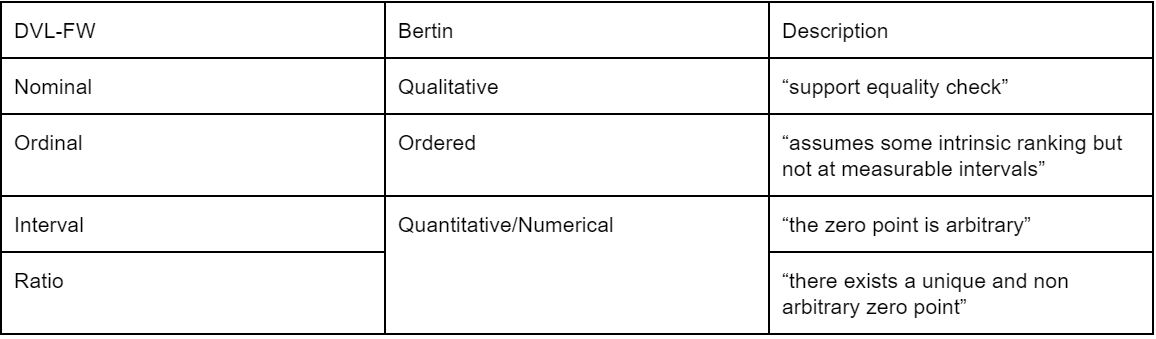
\includegraphics[width=.9\linewidth]{images/borner19_logical_operations.png}
	\caption{Logical mathematical operations permissible for data per Borner2019's DVL-FW}
	\label{fig:borner2019_logical_ops}
\end{figure}

\begin{figure}[H]
	\centering
	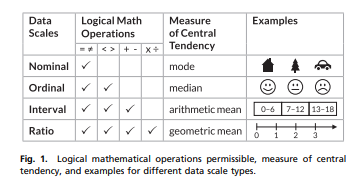
\includegraphics[width=.9\linewidth]{images/borner2019_figure1.png}
	\caption{Logical mathematical operations permissible, measure of central tendency, and examples for different data scale types (Borner2019)}
	\label{fig:borner2019_fig1}
\end{figure}

\begin{figure}[H]
	\centering
	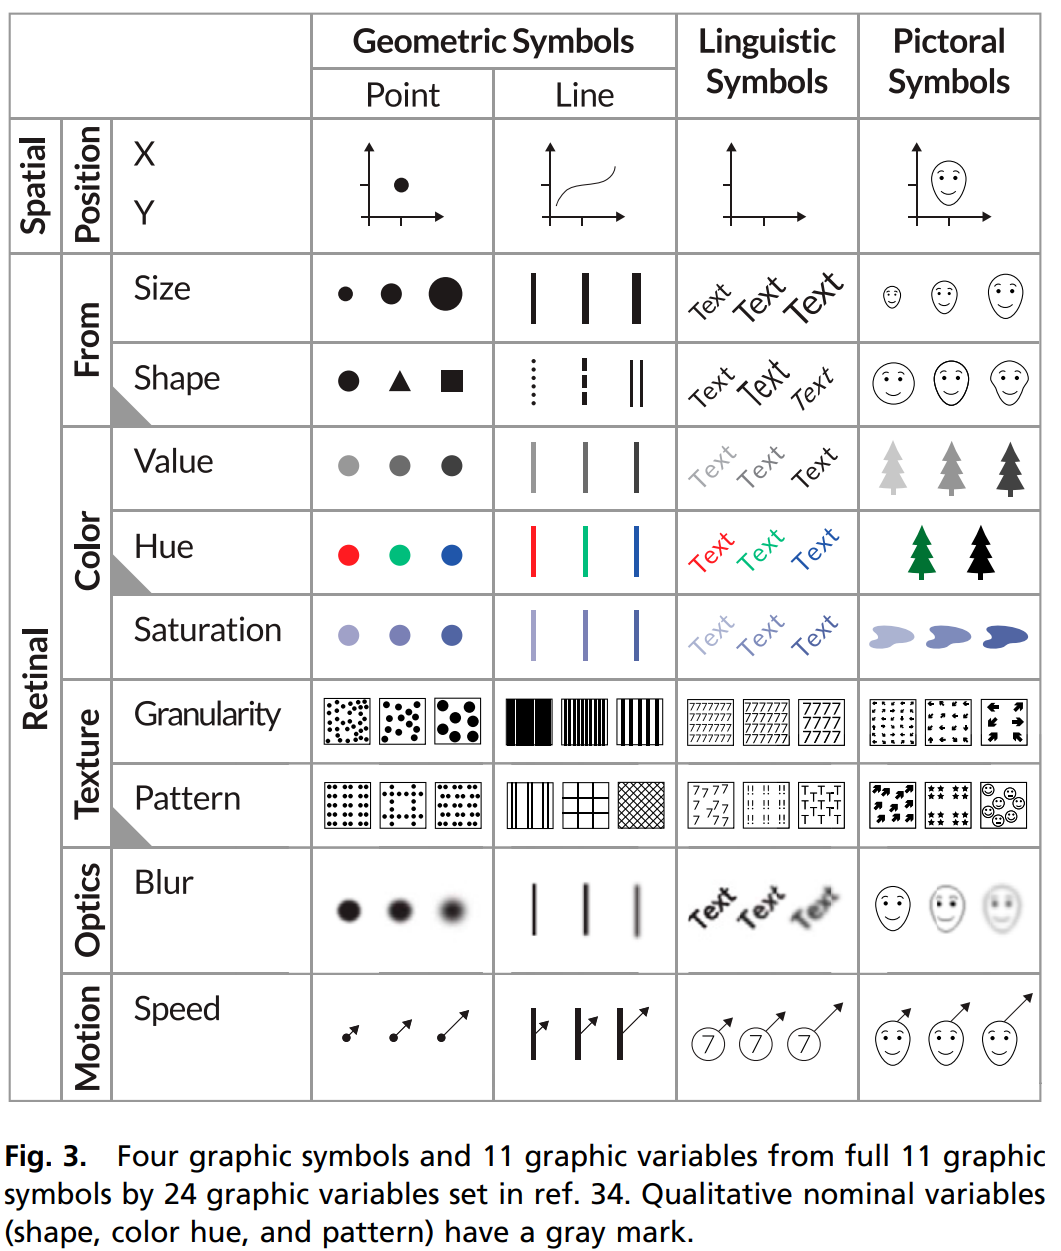
\includegraphics[width=.9\linewidth]{images/borner2019_figure3.png}
	\caption{Four graphic symbols and 11 graphic variables from full 11 graphic symbols by 24 graphic variables set in ref. 34. Qualitative nominal variables (shapre, color, hue, and pattern) have a gray mark. (Borner2019)}
	\label{fig:borner2019_fig3}
\end{figure}

Temporal folding \\

-{\color{orange}“With long, rapidly changing time series it can be difficult to see the subsets relevant to an event of interest. Many visualization excelat revealing periodic or cyclic phenomena through carefully chosen folded time scales, but non-periodic patterns can be obscured by a fixed time scale. When considering multiple event paris across sequences with varied interspersed gaps, it can be difficult to see the overall pattern of relationships between co-occurring events. THese problems are compounded by issues o data quality such as missing data, uncertainty in sensor or manual logs, inconsistency between sources with variou temporal granularities and level of accuracy, adn incorrect timestamps.”\cite{Zhang2019}}\\
-{\color{orange}“Temporal folding, or splitting, a sequence into periodic units like hours, weeks, months or years can be used to find cyclic phenomena. Folding can reduce pattern variety facilitating visual analysis.”\cite{Zhang2019}}\\
-{\color{orange}“Aligning sequences by sentinel events of interest helps users identify precursor, co-occurring, and aftereffect events… When aligned by a single event we can maintain a consistent time scale between folded or reconfigured units of event sequences. However, it can be valuable to explore the sequence between two separate sentinel events.”\cite{Zhang2019}}\\

%%%%%
\newpage
\section{Preliminary specification} \label{appendix:organization}
\begin{figure}[H]
	\centering
	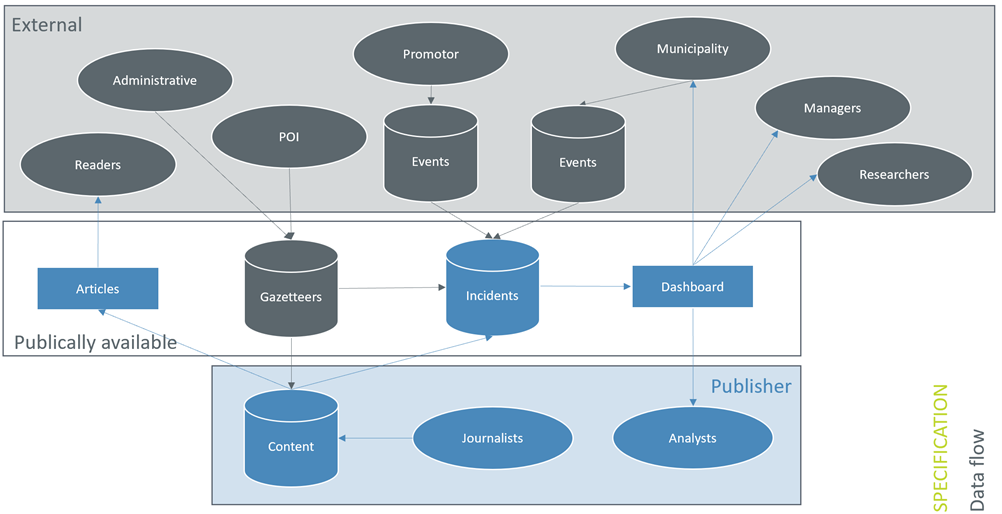
\includegraphics[width=.9\linewidth]{images/information_flow.png}
	\caption{Preliminary data and information flow}
	\label{fig:info_flow}
\end{figure}

\begin{figure}[H]
	\centering
	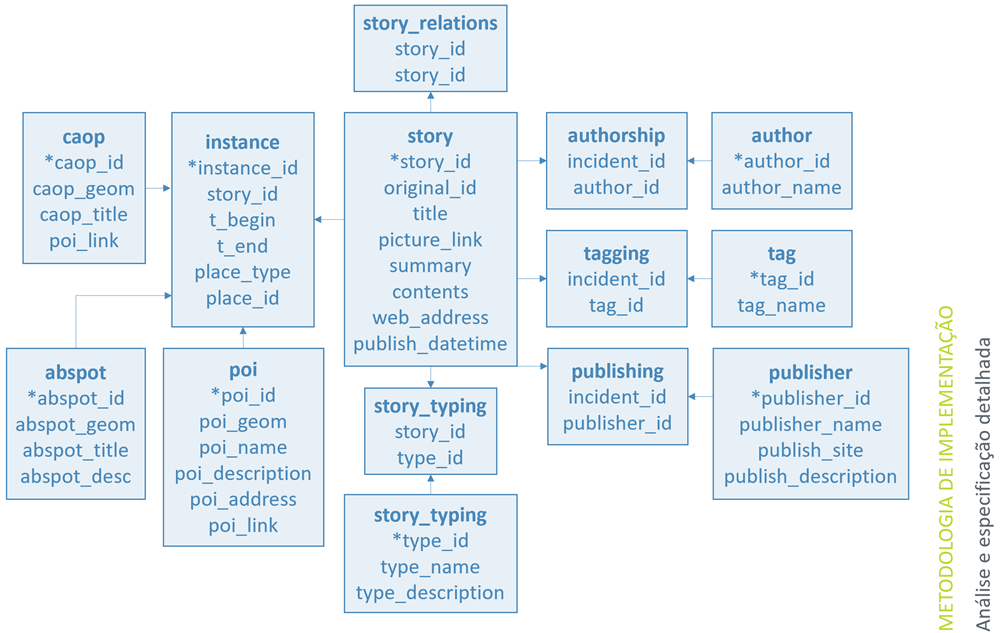
\includegraphics[width=.9\linewidth]{images/data_model.png}
	\caption{Preliminary data model fo the spatial database}
	\label{fig:data_model}
\end{figure}

\begin{figure}[H]
	\centering
	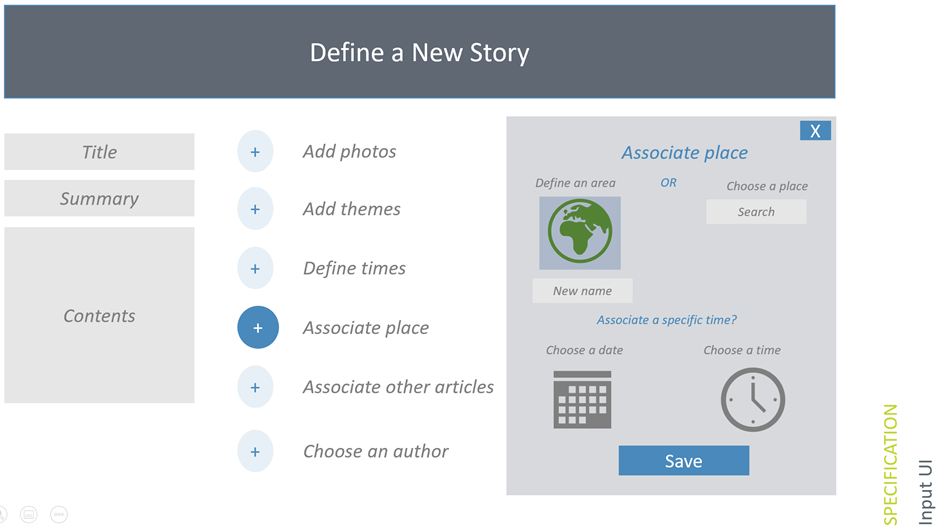
\includegraphics[width=.9\linewidth]{images/input_layout.png}
	\caption{Preliminary \textit{Input} layout}
	\label{fig:input_ui}
\end{figure}

\begin{figure}[H]
	\centering
	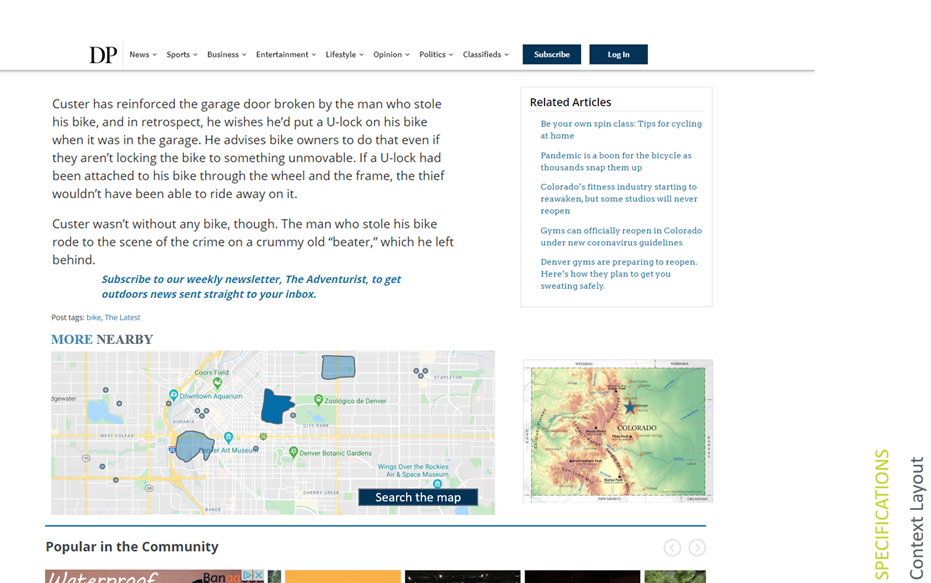
\includegraphics[width=.9\linewidth]{images/context_layout.png}
	\caption{Preliminary \textit{Context} layout}
	\label{fig:context_ui}
\end{figure}

\begin{figure}[H]
	\centering
	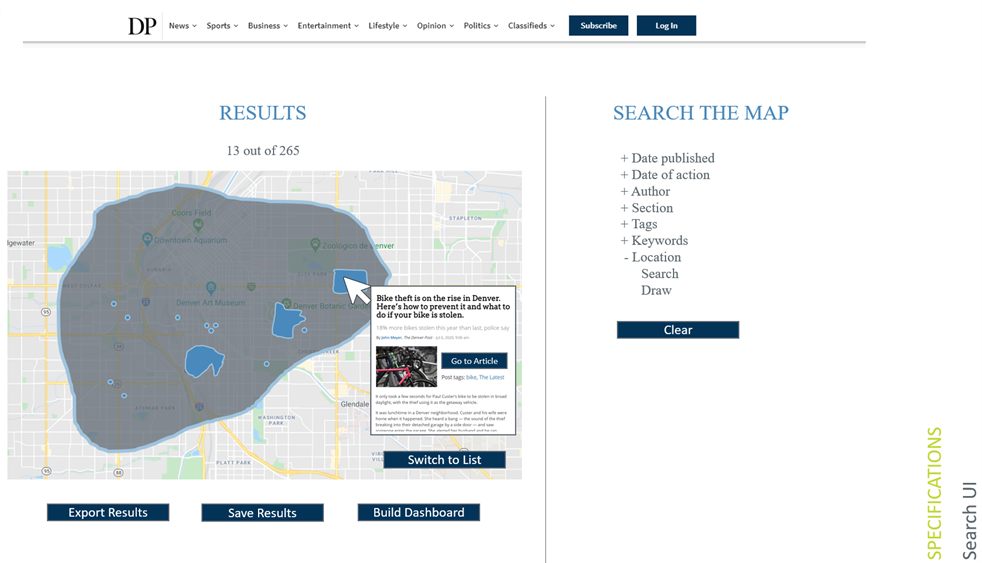
\includegraphics[width=.9\linewidth]{images/search_layout.png}
	\caption{Preliminary \textit{Search} layout}
	\label{fig:search_ui}
\end{figure}

\begin{figure}[H]
	\centering
	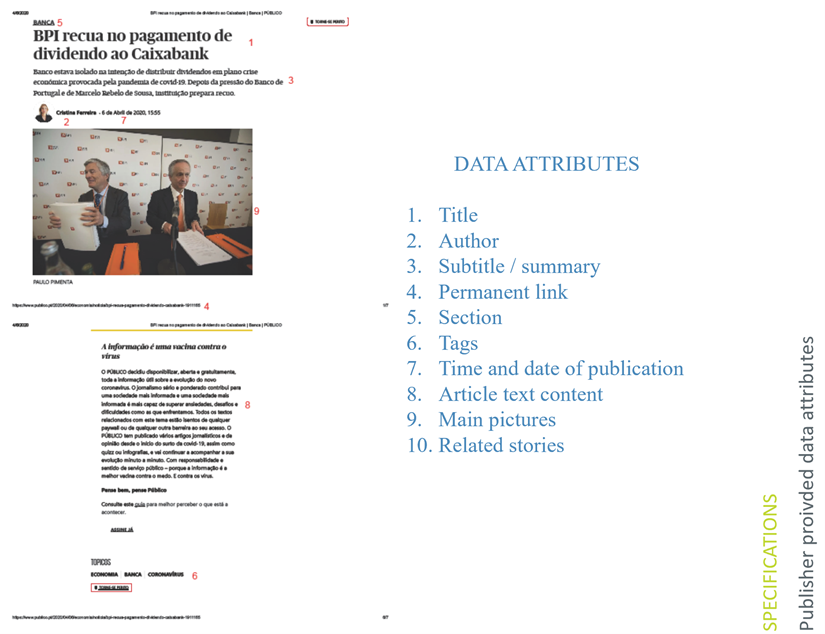
\includegraphics[width=.9\linewidth]{images/provided_attributes.png}
	\caption{Publisher provided data attributes}
	\label{fig:publisher_atts}
\end{figure}

%%%%%
\section{Example GUIs}
\begin{figure}[H]
	\centering
	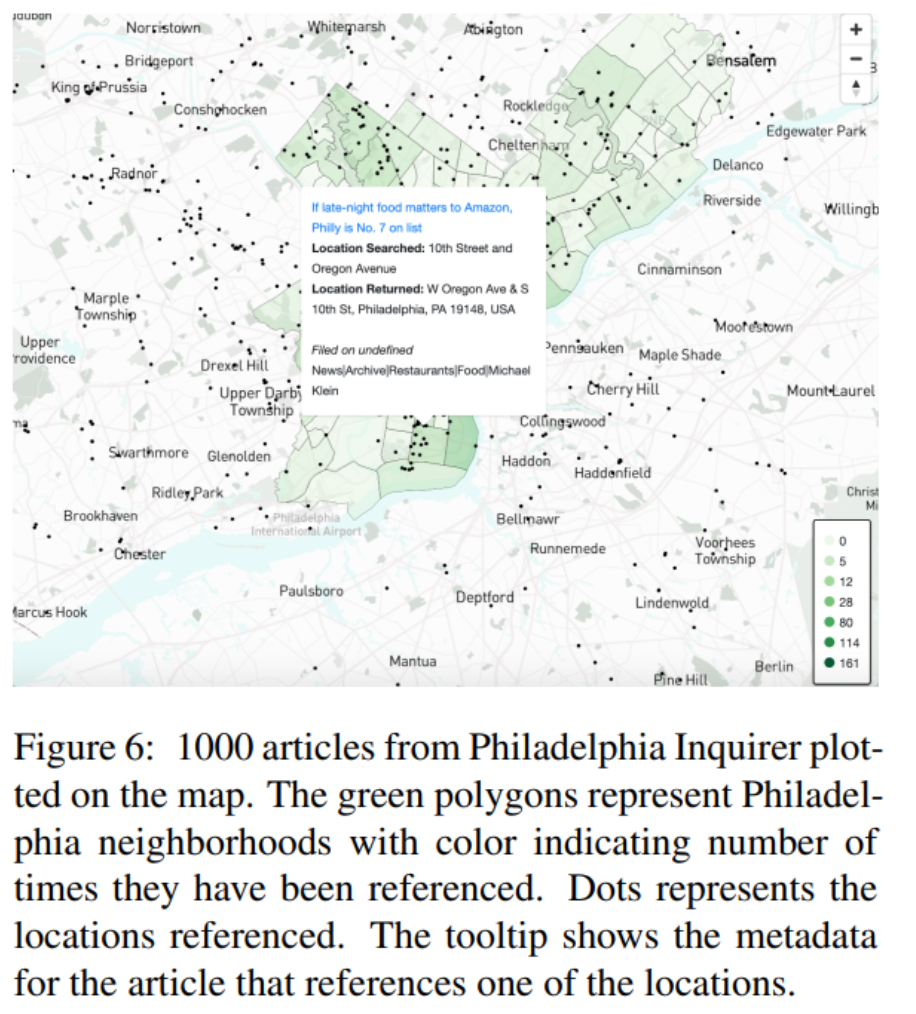
\includegraphics[width=.9\linewidth]{images/gupta2020_figure_6_mapped_article_layout.png}
	\caption{Mapped article layout (points) from Gupta2020}%\cite{Gupta2020}
	\label{fig:gupta2020_f6}
\end{figure}

\begin{figure}[H]
	\centering
	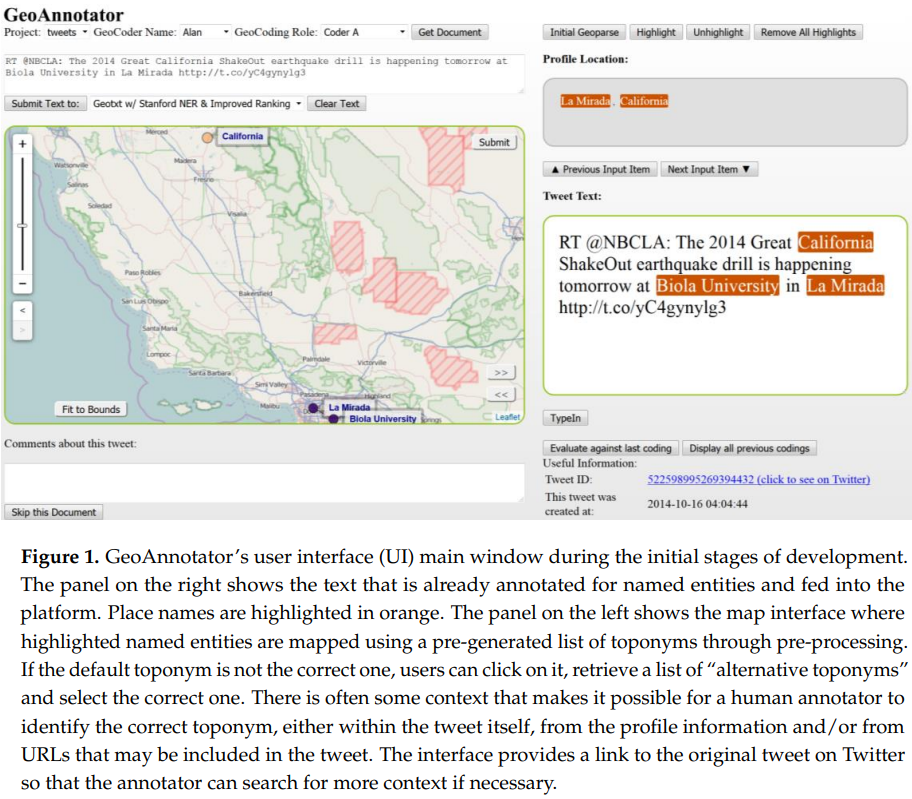
\includegraphics[width=.9\linewidth]{images/karimzadeh2019_figure1.png}
	\caption{Annotation via GeoAnnotator from Karimzadeh2019}%\cite{Karimzadeh2019}
	\label{fig:karimzadeh2019_f1}
\end{figure}

\begin{figure}[H]
	\centering
	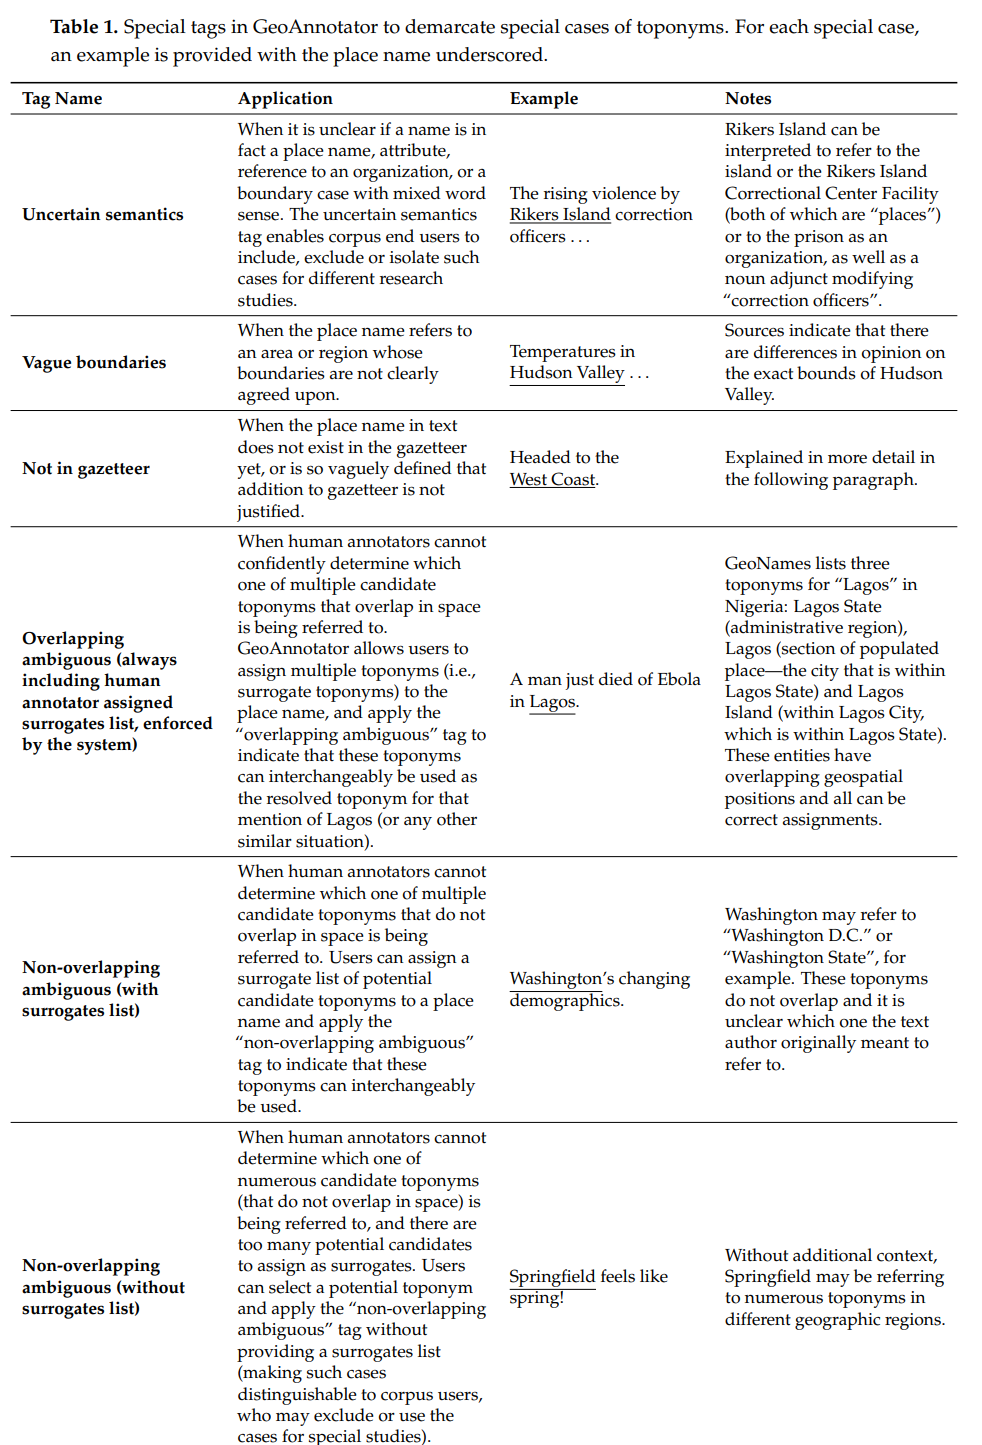
\includegraphics[width=.9\linewidth]{images/karimzadeh2019_table1.png}
	\caption{Annotation ambiguities from Karimzadeh2019}%\cite{Karimzadeh2019}
	\label{fig:karimzadeh2019_t1}
\end{figure}

\begin{figure}[H]
	\centering
	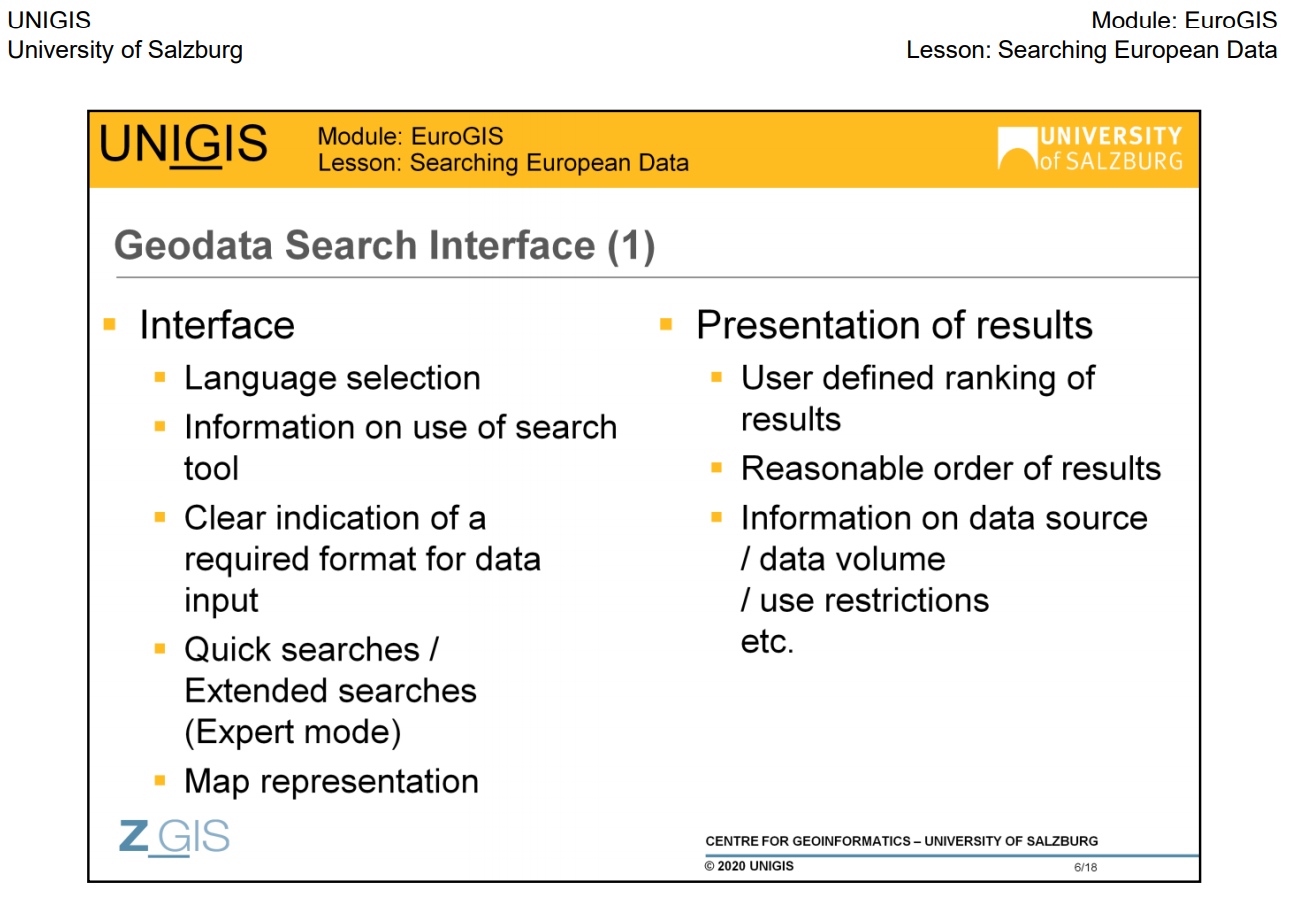
\includegraphics[width=.9\linewidth]{images/unigis_geodatasearch.png}
	\caption{Geodata Search Interface from Eisl2020}%\cite{Eisl2020}
	\label{fig:Eisl2020_f}
\end{figure}


\section{Example Architectures}
\begin{figure}[H]
	\centering
	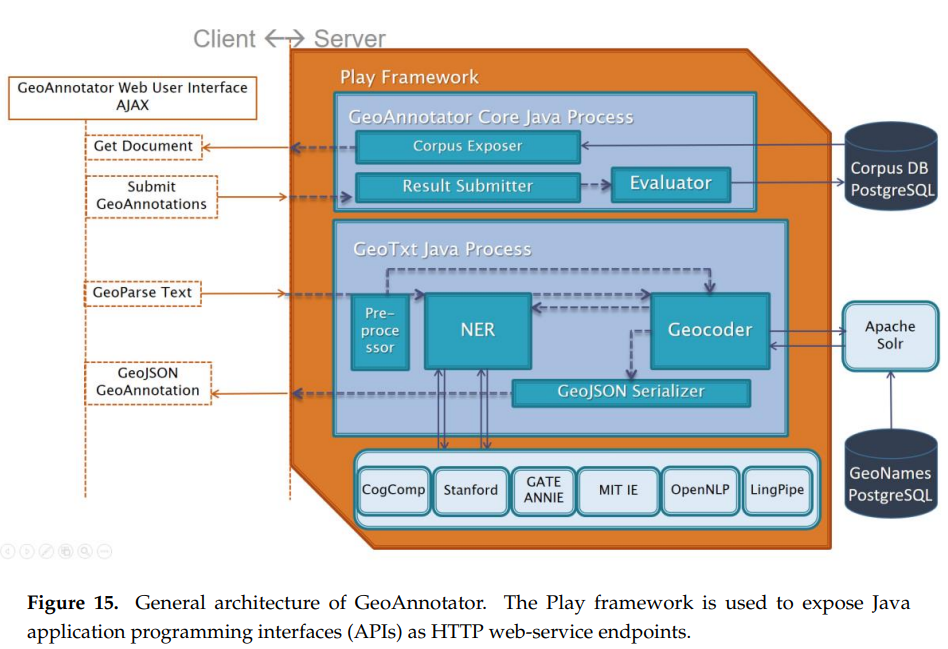
\includegraphics[width=.9\linewidth]{images/karimzadeh2019_figure15.png}
	\caption{general architecture of geoannotator from Karimzadeh2019}%\cite{Karimzadeh2019}}
	\label{fig:karimzadeh2019_f15}
\end{figure}
-{\color{orange}Client server model: server implemented in Java, and client (UI) implemented as webpages (HTML5, CSS and JavaScript). “to be scalable and accessible on a web browser to many annotators.” Bootstrap to be for display size flexibility, leaflet for mapping, jquery/jQuery UI/Rangy for functional operations. Server: PostgreSQL dataabase, corpus exposer module, result submitter module, evaluator module\cite{Karimzadeh2019}}{\color{red}see section 4.2 for architecture description and inspiration}\\

\begin{figure}[H]
	\centering
	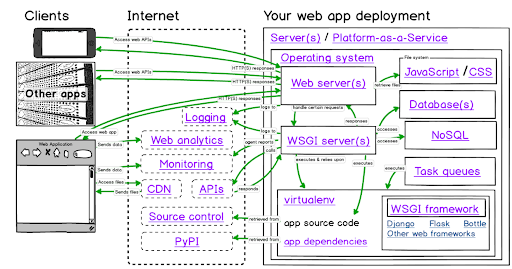
\includegraphics[width=.9\linewidth]{images/makai2020_fullstackdeploymentmap.png}
	\caption{Full stack deployment map from Makai2020}%\cite{Makai2020}
	\label{fig:Makai2020_f}
\end{figure}

\begin{figure}[H]
	\centering
	\includegraphics[width=.9\linewidth]{images/cai2016_figure5.png}
	\caption{Progressive georeferencing frameowrk from Cai2016}%\cite{Cai2016}
	\label{fig:cai2016_f5}
\end{figure}

\section{User stories}
\subsection{Micronews Portal}\cite{Carvalho2020}
- Uses Wordpress and NewsPack to publish news stories\\
- Require a plugin for incorpating main brands of maps (google maps, infogram, mapquest, storymaps, etc.)\\
- Uses geogrpahical data thatalready exists and is accessed. Want to understand which areas in Lisbon have more traffic crossing, number of stories, super markets, etc.\\
- Want to pull in elements from Maps.Me\\
- Have concerns about exposing which areas are covered versus not (news desserts)\\
- How do you connect with people in different areas: news letters vs. push alerts. Notifying of incidents in areas of interest/proximity. Frustrations with push alert communication.\\
- Seek to map geographic infomration in the website: a visualization of incidents occurring on a map. All content georefereced in and around Lisbon.\\
- Have three jouranlists in the field and data from the municipality\\
- References:
\begin{itemize}
	\item functionality of In Your Area to apply to communication of covid cases per area
	\item Oriental: orienting people in the middle east
\end{itemize}
- Lisbon data
\begin{itemize}
	\item {\color{orange}Access of juntas de freguesias.  All data comes from City hall. Covid data come from health minister}
	\item {\color{orange} Usability: many people don’t know the covid situation in their neighborhood. Are there 2 or 200 cases? TOOL DEVELOPED INFO APPLICATION STUDY. COVID specific: map cases AND news AND nursing homes AND layered data.}
	\item \href{https://www.lisboa.pt/fileadmin/cidade_temas/habitacao/listas/PRA3_lista_candidatos_sorteados_habitacao.pdf}{Lisboa data: Programa renda acessível}
\end{itemize}

%{\color{red} Include specifications matrix}

%\newpage
%\section{Relevant coursework}
%\begin{itemize}
%	\item{} Cartographic sciences
%	\item{} Geographic information standards
%	\item{} Geospatial intelligence (GEOINT)
%	\item{} Geo-statistics
%	\item{} Geospatial data mining
%	\item{} Modeling in GIS
%	\item{} GIS in organization
%	\item{} Open software and programming in GIS
%	\item{} Geographic databases and geospatial web services
%	\item{} Geographic information system
%	\item{} Information technology in cities (I and II)
%	\item{} Mobile and ubiquitous computing
%	\item{} Sustainable cities
%	\item{} Urban analytics
%	\item{} Remote sensing
%	\item{} Cybersecurity
%	\item{} Big data
%\end{itemize}
\end{appendices}

%%% SUMMARY

%\newpage
%\section*{Quick Description}
%The project is a set of tools that allow journalists/government/officials to georeference and timestamp their articles/documentation so that they can be spatially, temporally, and thematically searched by a variety of users. The hope is that this will bring additional context to local’s about their community via a familiar interface (a lá AirBnB, googlemaps, etc.), as well as more nuanced monitoring tools via spatial dashboards. Basically, it’s a geoportal that enables users better searchability to access already publicly available resources through querying tools that have already become the status quo in other industries.
%
%
%\newpage
%\section*{Applications}\label{sec:applications}
%Beyond the direct use of the tools being developed, there are opportunities to leverage the system as a geoportal, extracting information for more specific applications with geospatial new element. The toolset is intended to provide free and open access to the data contained within, with APIs providing means for other applications to incorporate the data for their own purposes. Several examples are illustrated below:
%
%\begin{enumerate}
%	\item Lisbon, PT: A website to inform citizens on the distribution of COVID within the city limits. A development team obtains i) locations of hospitals and nursing homes, locations of vital businesses (markets, pharmacies, gas stations, etc.), and boundaries of freguesias from Lisboa Aberta (open data portal managed by CML); ii) news stories related to covid (results from the toolset filtered to Lisbon Municipality boundary and 'COVID' tags); and iii) aggregation (by freguesia) of active COVID cases as well as identified hotspot areas from the Ministry of Health.  Users are able to monitor their locations of interest (home, work, play, family, and friends) in terms of relative cases compared to the rest of the city and adjust their behavior in those areas accordingly.  Trips to vital services can be planned more effectively. City officials may also identify areas of poor coverage for vital services and temporarily support those areas with access to walkable points of pickup for food an other necessities.
%	\item Campolide, Lisboa, PT: An environmental task force for the freguesia Campolide seeks to better understand the ecological situation in their community.  Their team incorporates i) news stories within the Campolide boundary filtered to the 'ECO' tag, all mentions of keywords 'JARDIM', 'ESPACO VERDE', 'ECOSYSTEMA', 'QUALIDADE DA VIDA', and temporal range of the last year (17 Nov 2019 to 16 Nov 2020); ii) location of green spaces within the freguesia from Lisboa Aberta; iii) pollution and trash data from other sources; iv) citizen interview results. The task force can then perform the necessary statistical analysis to determine areas requiring intervention, or identify those areas to highlight in upcoming reports on successful green spaces within the community, or to learn about new grassroots initiatives to support.
%	\item Berlin, Germany: A research team is searching for statistics on the effect of the Spanish flu in Lisbon, Portugal.  They are not well-versed with the study area nor with the portuguese language.  They use the toolset to segretate their own study areas (not adhering to current or previous administrative boundaries of freguesias) within the city limits by drawing polygons over the reigon and setting a temporal content filter to January 1918 to December 1920, with tags 'DOENTE' and 'GRIPE ESPANHOLA', and filter this again to publish dates of each pre-2020 and 2020.  They incorporate this into their own study methods.  They are able to visualize the distribution of results of each query on a map, adding to their understanding of the coverage of each topic.
%\end{enumerate}


\end{document}